\documentclass[]{beamer}
\usetheme{Dresden}
% \useoutertheme{split}

\usepackage{color}
\usepackage{graphicx}
\usepackage{listings}
\usepackage{lmodern} %% allow bold keywords
\usepackage{menukeys}
\usepackage{qtree}

\definecolor{darkgreen}{rgb}{0,0.5,0}
\definecolor{lightblue}{rgb}{0.2,0.2,1}

\lstset{language=Java,
	basicstyle=\ttfamily\footnotesize,
	keywordstyle=\color{purple},
	commentstyle=\color{darkgreen},
	numberstyle=\tiny\color{gray},
	stringstyle=\color{blue},
	tabsize=4,
	showstringspaces=false,
	breaklines=true,
	keepspaces=true,
	numbers=left,
	escapechar=@
}

\title{Java}
\subtitle{Object-Oriented Programming}
\author{Nico Westerbeck}
\date{\today}

\tikzset{
  every overlay node/.style={
    draw=black,fill=white,rounded corners,anchor=north west,
  },
}
% Usage:
% \tikzoverlay at (-1cm,-5cm) {content};
% or
% \tikzoverlay[text width=5cm] at (-1cm,-5cm) {content};
\def\tikzoverlay{%
   \tikz[baseline,overlay]\node[every overlay node]
}%

\lstset{language=Java,
	basicstyle=\ttfamily\footnotesize,
	keywordstyle=\color{purple},
	commentstyle=\color{darkgreen},
	numberstyle=\tiny\color{gray},
	stringstyle=\color{blue},
	tabsize=4,
	showstringspaces=false,
	breaklines=true,
	keepspaces=true,
	numbers=left,
	escapechar=§
}

\begin{document}

\begin{frame}
\titlepage
\end{frame}
\begin{frame}{Overview}
\tableofcontents
\end{frame}

\section{Introduction}
\subsection{Recalling last session}
\begin{frame}{Java-tools}
	Datatypes
	\begin{itemize}
		\item int, long
		\item float, double
		\item String
	\end{itemize}
	Control statemenets
	\begin{itemize}
		\item if, else if, else
		\item while
		\item for
	\end{itemize}
\end{frame}

\begin{frame}{Mind-tools}
	\begin{center}
		{\huge Think in code!}
		% Key of imperative programming: Breaking down a complex command into a sequence of easier ones
		% Know, which commands already exist
		% Know, what you have to store (variables)
		
		% Tasks for audience to answer "in code":
		% Example: Count the number of 'e' in a String
		% Remove all uppercase letters within a String and add them to the end of that String
		% Check if Random class is fair when generating numbers between 0 and 5
		% Take a speed in km/h and output the miles/h version and vice versa
		% Check if a password-String contains a number, a lowercase-letter and an uppercase letter
		% Check if a (small) number is a prime number
		% Check if String is palindrome
		% Zahlenraten!
	\end{center}
\end{frame}

\subsection{Think in Objects}

\begin{frame}{}
	\begin{center}
		\uncover<1-2>{\huge Think in objects!}
		% The representation of a certain class of contributors in a problem.
		% What is a
		
		% Instance vs Object
		
		\uncover<2-2>{\vspace{0.5cm}\normalsize The representation of a certain contributor to a problem}
		
		% Problem:
		%	- Your task, that you want to solve with Java
		%	- Since problem is negative, let's call it challenge ;)
		
		% Contributors:
		%	- Things that you need to think about/that get noted if you write down your problem
		%	- Have a state and a behaviour within the challenge
		%	- Fairytale-rule: Everything that could get a name, if you make a fairytale out of your challenge, is an object

		% Representation:
		% 	- Limited to the possibilities of the programming language:
		% 	- State = Fields, Variables
		%	- Behaviour = Methods
		%	- Can only be an instance of a class
		%	- Dafuq is a class and an instance? Later...
		
		% Let them identify some objects on next slides:
	\end{center}
\end{frame}

\section{Identifying objects}
\subsection{Examples}

\begin{frame}{}
	\begin{center}
		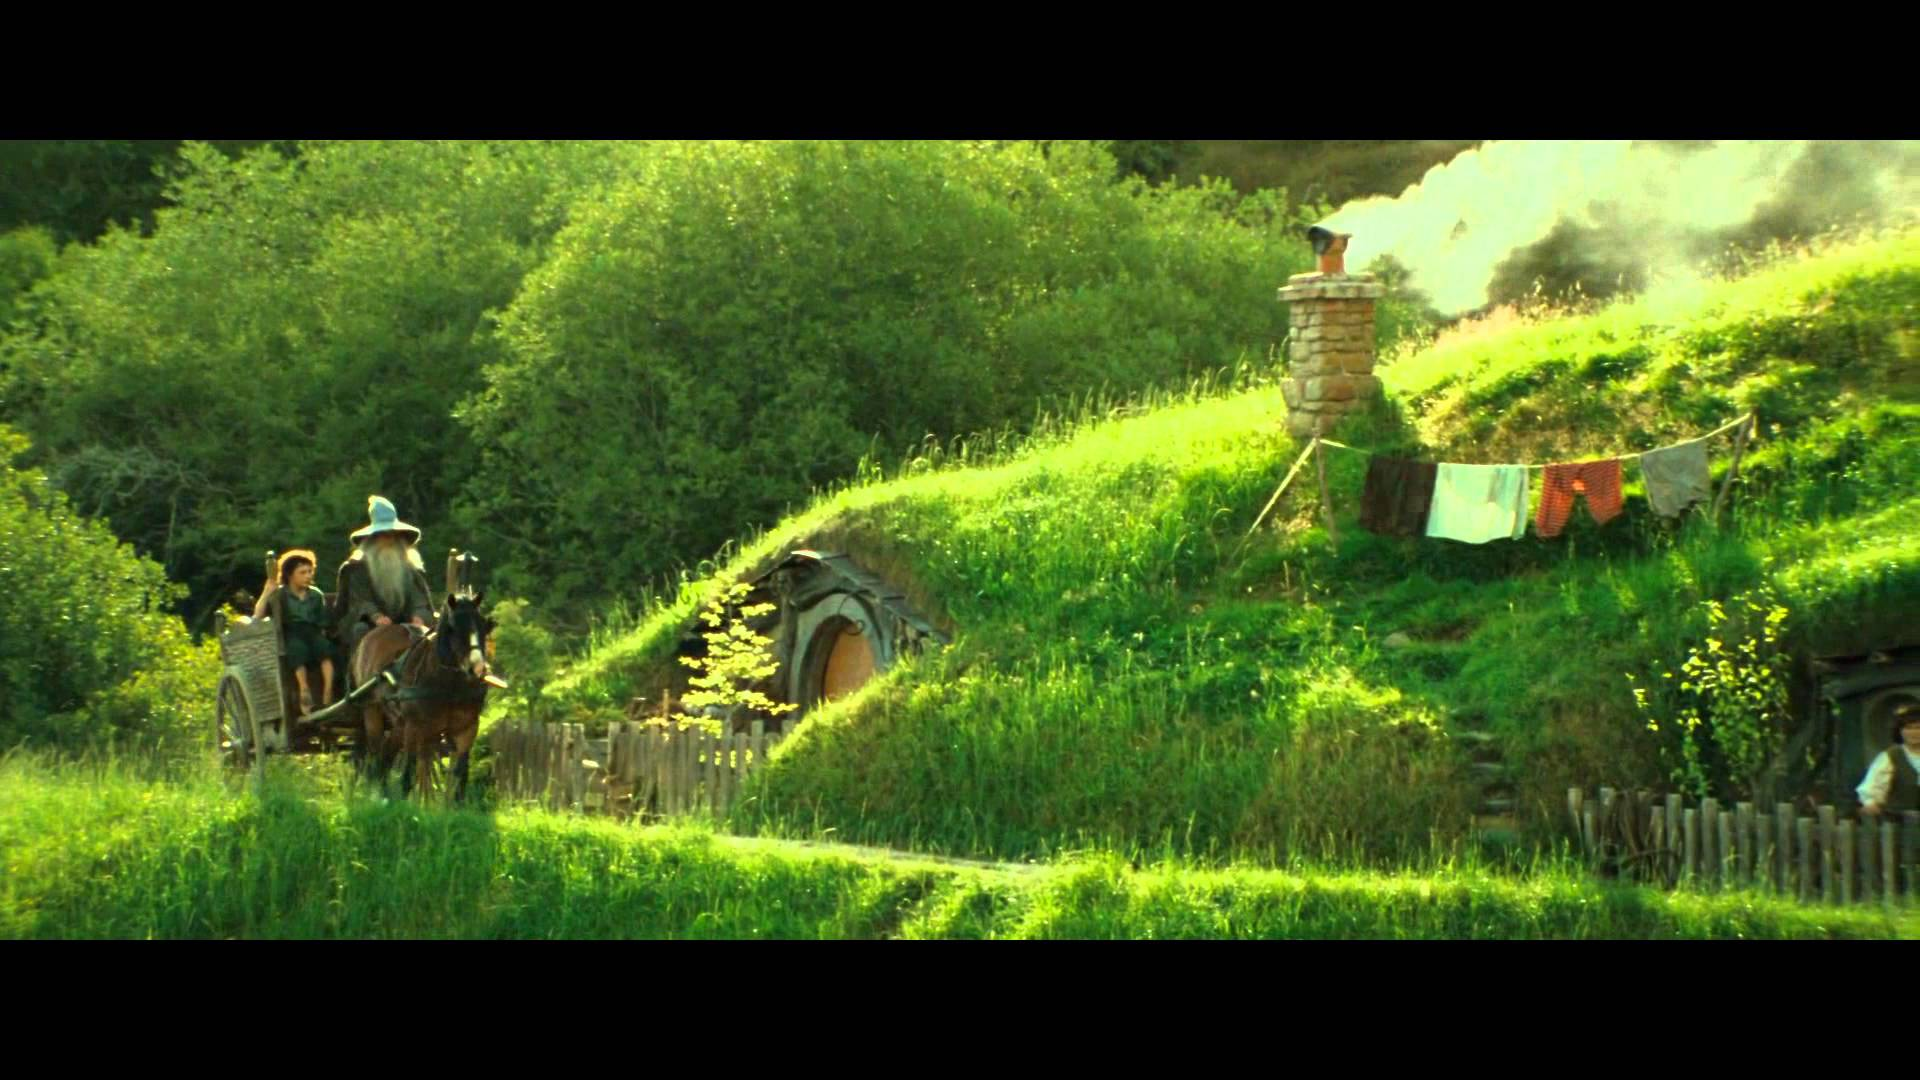
\includegraphics[width=11cm]{res/lotr-shire.jpg}
	\end{center}
\end{frame}

\begin{frame}{}
	\begin{center}
		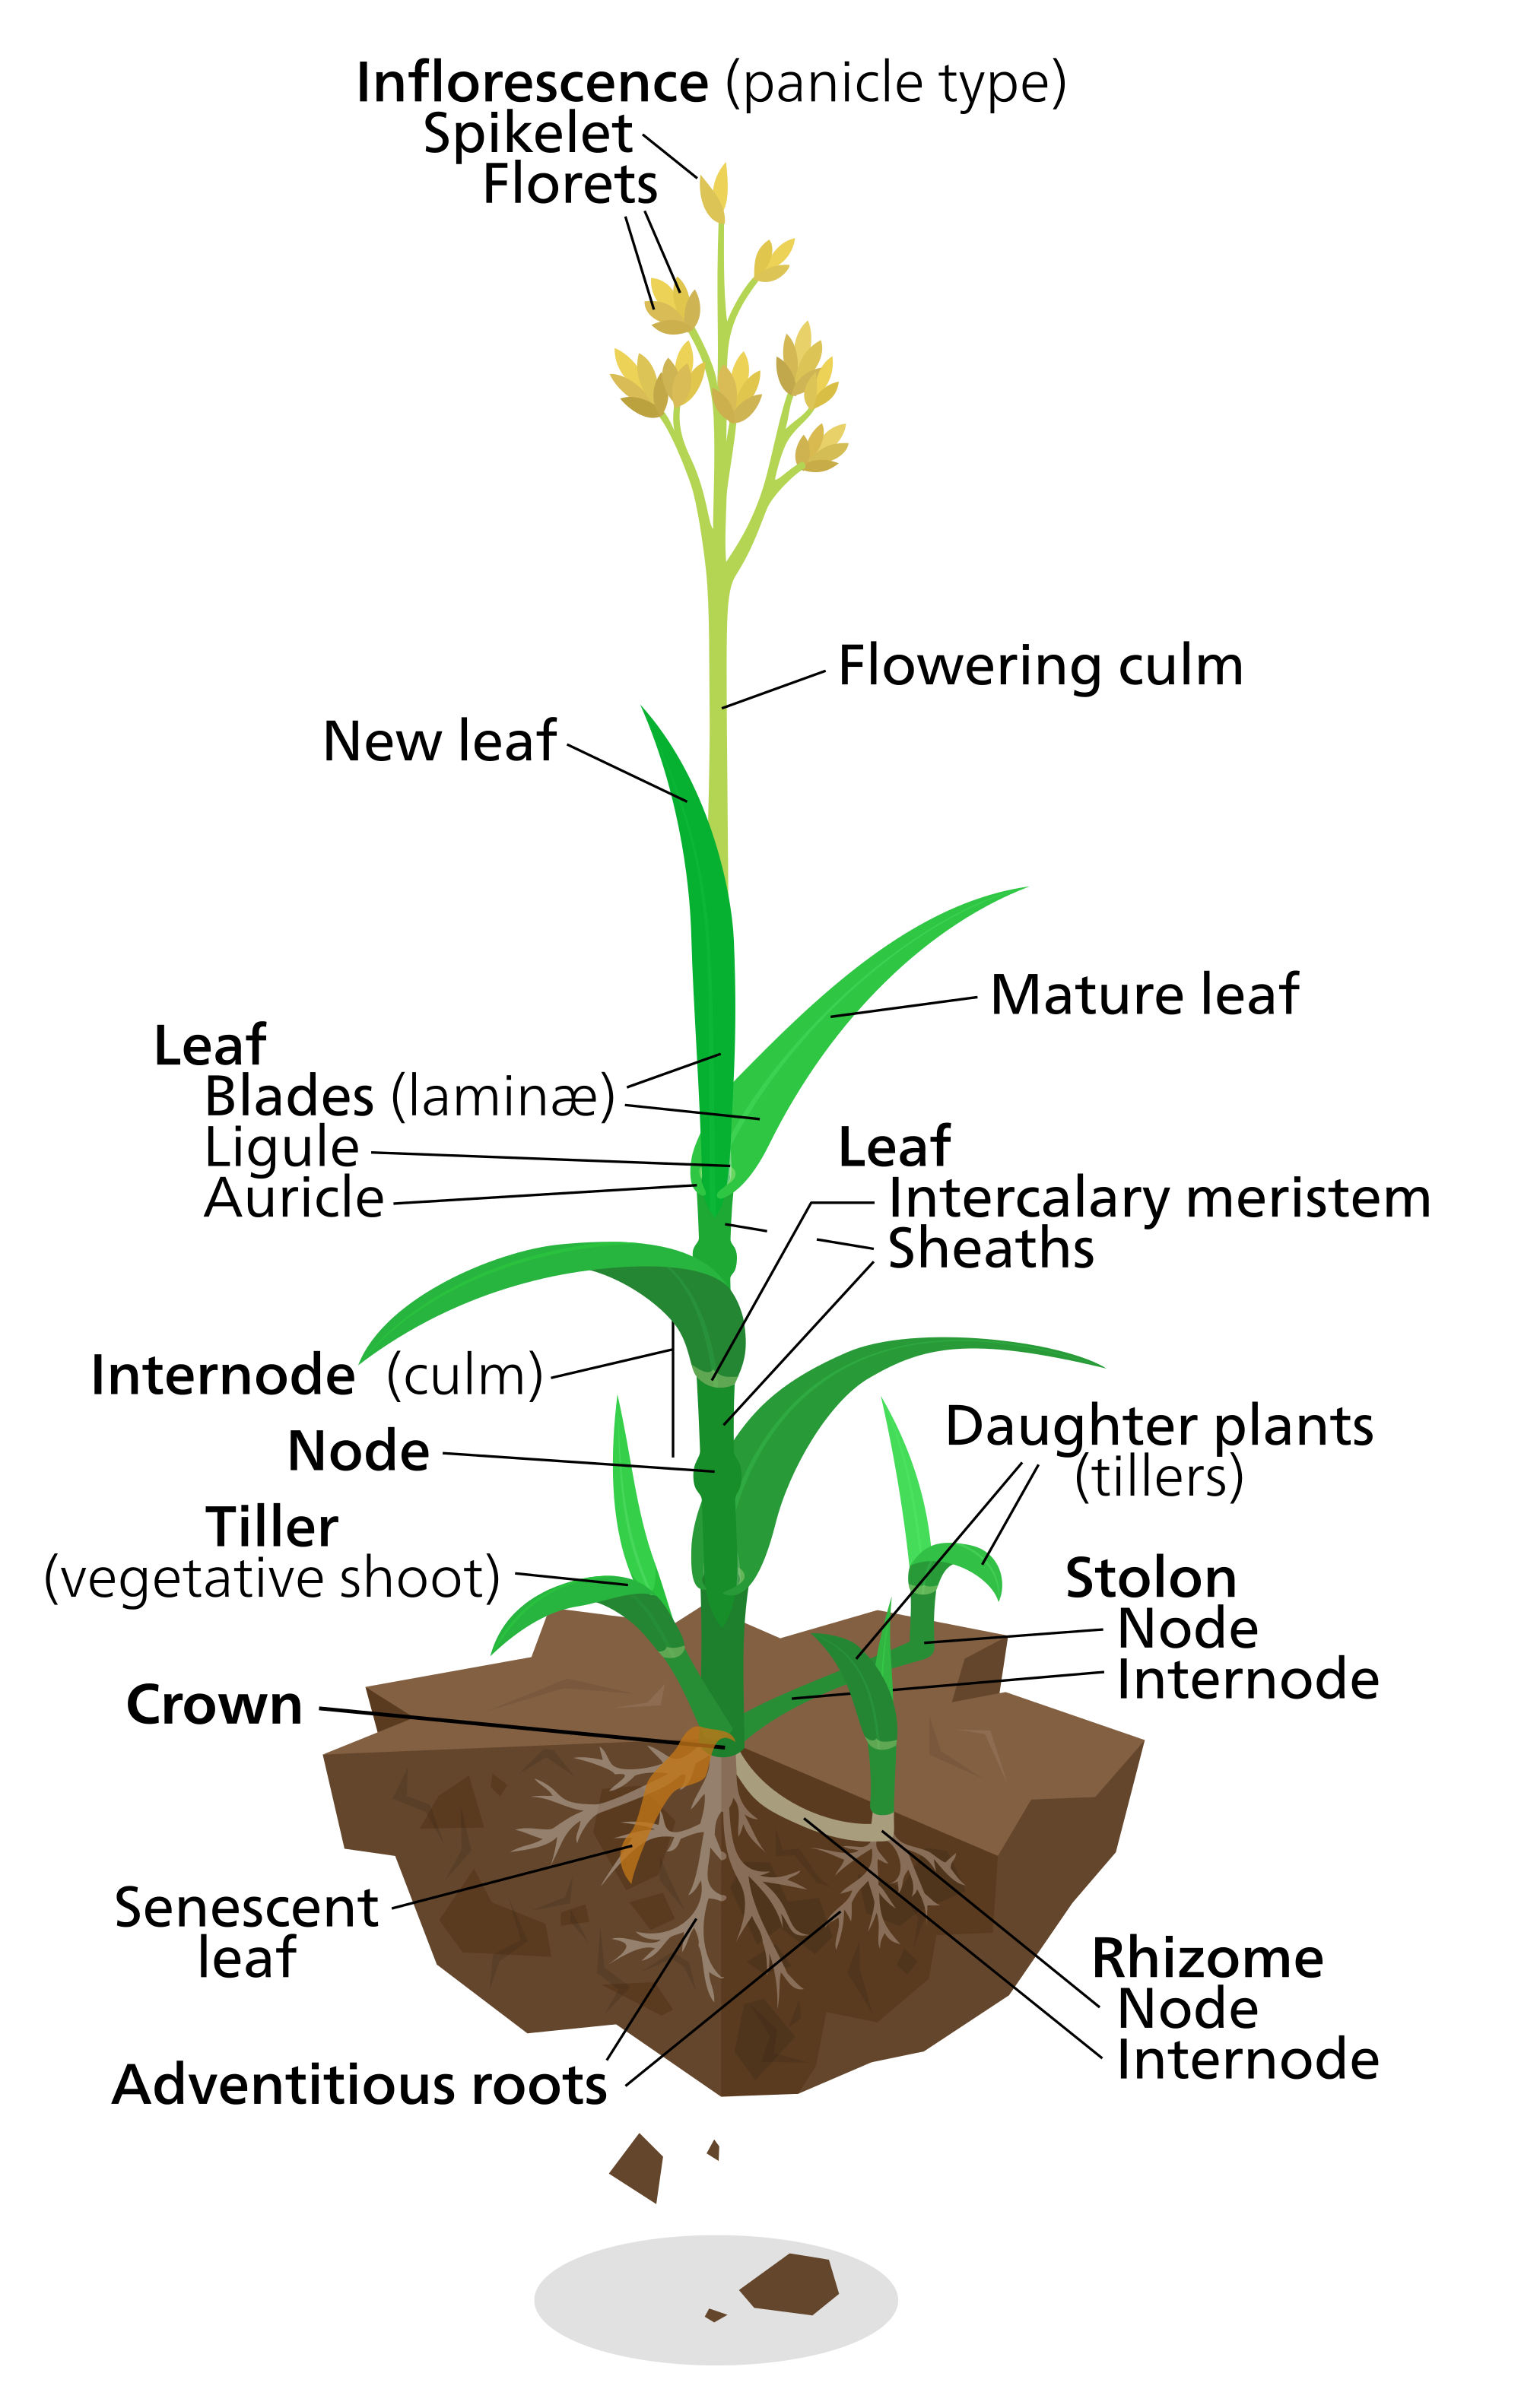
\includegraphics[height=7cm]{res/grass-plant.png}
	\end{center}
\end{frame}

\begin{frame}{}
	\begin{center}
		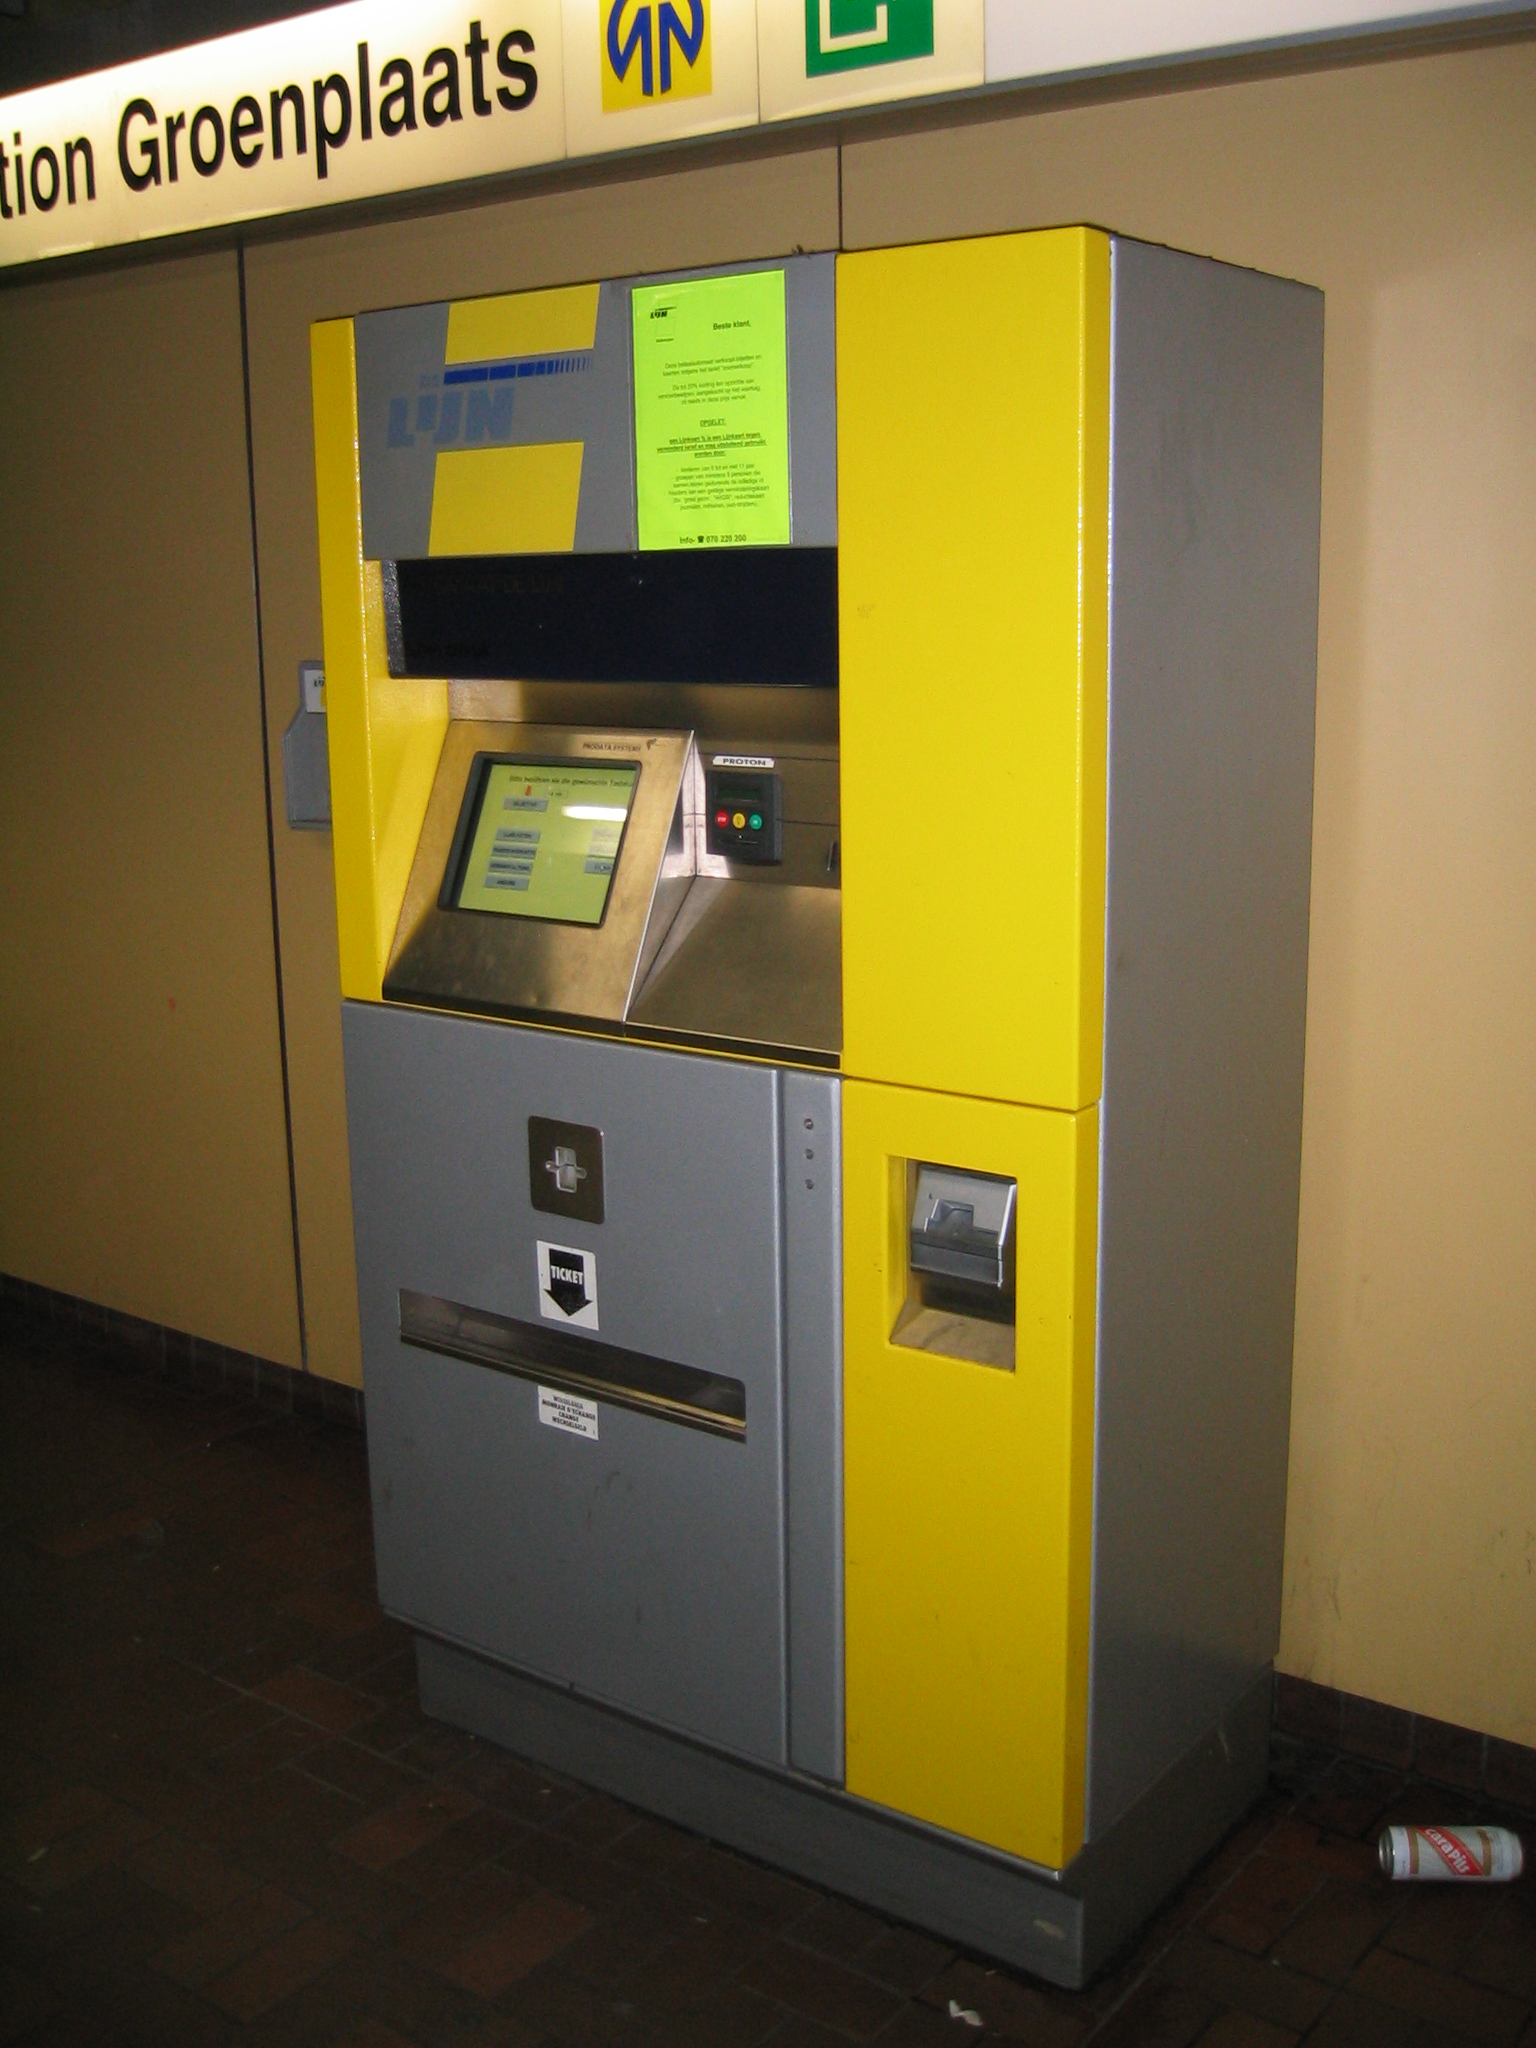
\includegraphics[height=7cm]{res/ticket-vending-machine.jpg}
	\end{center}
\end{frame}

\subsection{Class vs Instance}

\begin{frame}{}
	\begin{center}
		{\huge Class vs Instances - the Peter-rule}
		%	Object-instance can be named Peter
		%	Object-class can be put into an encyclopedia
		% Example: (Show ticket, name it Peter) is an instance, Viererticket is a class
		%   Class is like a blueprint, Instance is the existing object
		%	This is why instance is sometimes refered to as an object
		% Go back to images and let them identify classes
		% Then let them identify classes in a student enrollment system (Student should be amongh that)
	\end{center}
\end{frame}

\section{OOP in Java}
\subsection{General information}

\begin{frame}[fragile]{Class \emph{Student}}
\begin{lstlisting}
public class Student {

	// Attributes
	private String name; 
	private int matriculationNumber; 
	
	/**
	 * Changes the name
	 * @param name The new name of the student
	 */
	public void changeName(String name) {
		this.name = name;
	}
}
\end{lstlisting}

% What is visible here:
% Attributes store the state of the object
% Methods implement the behaviour of the object


\end{frame}

\begin{frame}[fragile]{Creation}
	We learned how to declare and assign a primitive datatype.
	\begin{lstlisting}
	    int a; // declare a
	    a = 273; // assign 273 to a
	\end{lstlisting} 
	The creation of an object works similar.
	\begin{lstlisting}
	    Student example; // declare example
	    example = new Student(); // create an instance of Student
	\end{lstlisting}
	The \textbf{object} derived from a \textbf{class} is also called \textbf{instance}.
	The variable\footnote{in this listing \emph{example}} is called the \textbf{reference}.
\end{frame}

\subsection{Methods}
\begin{frame}[fragile]{Calling a Method}
	\begin{lstlisting}
	public class Student {
		private String name;
	
	    public void changeName(String newName) {
			name = newName;
	    }
	    
	    public void printName() {
	        System.out.println(name);
	    }
	}
	\end{lstlisting}
	The class \emph{Student} has two methods: \emph{void printTimetable()} and \emph{void printName()}.
\end{frame}

\begin{frame}[fragile]{Calling a Method}
\begin{lstlisting}
	public class Main {
	    
	    public static void main(String[] args) {
	        Student example = new Student(); // creation
	        example.changeName("Jane"); // method call
	        example.printName(); // Prints "Jane"
	    }
	}
	\end{lstlisting}
	You can call a method of an object after its creation with \textbf{reference.methodName();}.
\end{frame}

\begin{frame}[fragile]{Calling a Method}
\begin{lstlisting}
	public class Student {
		private String name;
	
	    public void changeName(String newName) {
			name = newName;
			printName();   // Call own method
			this.printName(); // Or this way
	    }
	    
	    public void printName() {
	        System.out.println(name);
	    }
	}
	\end{lstlisting}
	You can call a method of the own object by simply writing \textbf{methodName();} or \textbf{this.methodName();}
\end{frame}

\begin{frame}[fragile]{Methods with Arguments}
	You can call a method with e.g. two arguments via \texttt{methodName(arg1, arg2)}.
	\begin{lstlisting}
	public class Calc {
	
	    public void add(int summand1, int summand2) {
	        System.out.println(summand1 + summand2);
	    }
	    
	    public static void main(String[] args) {
	        int summandA = 1;
	        int summandB = 2;
	        Calc calculator = new Calc();
	        System.out.print("1 + 2 = ");
	        calculator.add(summandA, summandB); // prints: 3
	    }
	}
	\end{lstlisting}
\end{frame}

\subsection{Return Value}
\begin{frame}[fragile]{Methods with Return Value}
	A method without a return value is indicated by \textbf{void}:
	\begin{lstlisting}
	public void add(int summand1, int summand2) {
	    System.out.println(summand1 + summand2);
	}
	\end{lstlisting}
	A method with an \textbf{int} as return value:
	\begin{lstlisting}
	public int add(int summand1, int summand2) {
	    return summand1 + summand2;
	}
	\end{lstlisting}
	% TODO explain return statement
\end{frame}

\begin{frame}[fragile]{Calling Methods with a return value}
	\begin{lstlisting}
	public class Calc {
	
	    public int add(int summand1, int summand2) {
	        return summand1 + summand2;
	    }
	    
	    public static void main(String[] args) {
	        Calc calculator = new Calc();
	        int sum = calculator.add(3, 8);
	        System.out.print("3 + 8 = " + sum); // prints: 3 + 8 = 11
	    }
	}
	\end{lstlisting}
\end{frame}

\subsection{Constructor}

\begin{frame}[fragile]{Constructors}
	\begin{lstlisting}
	public class Calc {
		private int summand1;
		private int summand2;
	
	    public Calc() {
			summand1 = 0;
			summand2 = 0;
	    }
	}
	\end{lstlisting}
	A constructor gets called upon creation of the object
\end{frame}

\begin{frame}[fragile]{Constructors with Arguments}
	\begin{lstlisting}
	public class Calc {
		private int summand1;
		private int summand2;
	
	    public Calc(int x, int y) {
			summand1 = x;
			summand2 = x;
	    }
	}
	[...]
	Calc myCalc = new Calc(7, 9);
	\end{lstlisting}
	A constructor can have Arguments aswell!
\end{frame}

\section{Conclusion}
\subsection{An Example}

\begin{frame}{An Example}
	You want to program an enrollment system, for a programming course. \\
	\vspace{1em}
	Your classes are:\\
	\begin{description}
		\item[student] who wants to attend the course
		\item[lesson] which is a part of the course
		\item[tutor] the guy with the bandshirt
		\item[room] where your lessons take place
		\item[\dots]
	\end{description}
% 	The more you think about it, the more complex this program becomes.
% 	Focus on the relevant things.
%	Think about how the objects can be in relation, this will be discussed later
%	Show prepared classes in Java
\end{frame}

\begin{frame}{Your task}

\begin{itemize}
	\item Hope for your tutor to send the classes he showed
	\item Open+compile them in Eclipse
	\item Look at them, find something I did not explain yet ;-)
	\item Add 3 more methods to any of the classes
	\item Add 3 more fields and use them in your methods
	\item Call at least 1 of the methods in a given one
\end{itemize}

\end{frame}


% \begin{frame}[fragile]{Class \emph{Student}}
% \begin{lstlisting}
% /**
%  * Main method
%  */
% public static void main(String[] args) {
% 	Student peter = new Student();
% 	peter.changeName("Peter");
% }
% \end{lstlisting}
% \end{frame}

\subsection{Credits}

\begin{frame}{Images stolen at:}
	\tiny
	\begin{itemize}
		\item \textbf{Shire image} Taken from film Lord of the Ring - The Fellowship of the Ring
		\item \textbf{Grass schema} By Thorsten Schmidt, via Wikimedia Commons
		\item \textbf{Ticket-vending-machine} By Thorsten Schmidt, via Wikimedia Commons
	\end{itemize}
	
\end{frame}

% Next lesson: Using classes provided in Java


\end{document}